% CA6001 technical report -- LaTeX source.
% Build from this folder:  latexmk -pdf main.tex   (see README.md)
% Prose lives in sections/*.tex; tables in tables/*.tex are generated by make_tables.py;
% figures are read from ../results/adaptive_v1/figures/ (generated by cpt_budget.report_figures).
\documentclass[12pt,a4paper]{article}

% ---------------------------------------------------------------- fonts and layout
\usepackage[T1]{fontenc}
\usepackage{amsmath,amssymb}
\usepackage{newtxtext,newtxmath}
\usepackage[a4paper,margin=2.54cm,footskip=1.0cm]{geometry}% as the course Word template
\usepackage{microtype}
\setlength{\parindent}{1.2em}
\setlength{\parskip}{0pt plus 1pt}
\linespread{1.0}

% ---------------------------------------------------------------- floats, tables, figures
\usepackage{graphicx}
\graphicspath{{../results/adaptive_v1/figures/}}
\usepackage{booktabs,tabularx,array,multirow}
\usepackage[font=small,labelfont=bf,labelsep=period,skip=4pt]{caption}
\usepackage{float}
\renewcommand{\topfraction}{0.9}
\renewcommand{\bottomfraction}{0.8}
\renewcommand{\textfraction}{0.07}
\renewcommand{\floatpagefraction}{0.8}
\setlength{\textfloatsep}{8pt plus 2pt minus 2pt}
\setlength{\floatsep}{6pt plus 2pt minus 2pt}
\setlength{\intextsep}{6pt plus 2pt minus 2pt}

% ---------------------------------------------------------------- headings and lists
\usepackage{titlesec}
\usepackage{xcolor}
\definecolor{head}{HTML}{1C3D5A}
\definecolor{muted}{HTML}{52514E}
\definecolor{codebg}{HTML}{F3F2EE}
\titleformat{\section}{\large\bfseries}{\thesection}{0.6em}{}
\titleformat{\subsection}{\normalsize\bfseries}{\thesubsection}{0.6em}{}
\titlespacing*{\section}{0pt}{9pt plus 2pt}{3pt}
\titlespacing*{\subsection}{0pt}{6pt plus 2pt}{2pt}
\usepackage{enumitem}
\setlist{nosep,leftmargin=1.2em,topsep=1pt}

% ---------------------------------------------------------------- code
\usepackage{listings}
\lstset{basicstyle=\ttfamily\footnotesize,backgroundcolor=\color{codebg},frame=none,
  columns=fullflexible,keepspaces=true,xleftmargin=0.6em,aboveskip=3pt,belowskip=3pt,
  commentstyle=\color{muted},language=Python,showstringspaces=false}
\lstdefinestyle{output}{language={},keywordstyle={}}

% ---------------------------------------------------------------- symbols and units
\usepackage{eurosym}
\newcommand{\qc}{\ensuremath{q_c}}
\newcommand{\Bfull}{\ensuremath{B_{\text{full}}}}
\newcommand{\Bseq}{\ensuremath{B_{\text{seq}}}}
\newcommand{\Padapt}{\ensuremath{P_{\text{adapt}}}}
\newcommand{\Nfull}{\ensuremath{N_{\text{full}}}}
\newcommand{\Nstop}{\ensuremath{N_{\text{stop}}}}
\newcommand{\eur}[1]{\textup{\euro{}#1}}% text-mode amount, safe inside math

% ---------------------------------------------------------------- references
\usepackage[style=apa,backend=biber]{biblatex}
\usepackage{csquotes}
\addbibresource{references.bib}
\renewcommand*{\bibfont}{\small}
\setlength{\bibitemsep}{0pt}

\usepackage[hidelinks]{hyperref}
\usepackage[capitalise,nameinlink,noabbrev]{cleveref}
\crefname{figure}{Figure}{Figures}
\Crefname{figure}{Figure}{Figures}

\begin{document}

% Cover page (not counted in the 10-page limit). Fill in the team table before submission.
\begin{titlepage}
\centering
\vspace*{2.2cm}
{\large\color{muted} CA6001 -- AI Algorithms Fundamentals \& Application\par}
{\color{muted} Group Project Technical Report\par}
\vspace{1.6cm}
{\LARGE\bfseries\color{head} Machine Learning--Guided Adaptive CPT Site Investigation\\[4pt]
and Economic Benefit Assessment\par}
\vspace{0.6cm}
{\large\color{muted} Predicting shallow cone-resistance profiles, choosing the next tests,\\
deciding when to stop, and pricing the outcome\par}
\vspace{1.8cm}

\begin{flushleft}
\textbf{Project Title:} Machine Learning--Guided Adaptive CPT Site Investigation and Economic Benefit Assessment\\[4pt]
\textbf{Course:} CA6001 AI Algorithms Fundamentals \& Application\\[4pt]
\textbf{Date:} October 2026\\[14pt]
\textbf{Student Names and Contributions:}\\[4pt]
\renewcommand{\arraystretch}{1.5}
\begin{tabularx}{\linewidth}{@{}p{4.6cm}p{3.0cm}X@{}}
\toprule
Name & Matriculation no. & Main contributions\\
\midrule
 & & \\
 & & \\
 & & \\
 & & \\
 & & \\
\bottomrule
\end{tabularx}
\end{flushleft}

\vfill
{\small\color{muted} Code, configuration and result files: project repository, package \texttt{cpt\_budget};
figures and tables in this report are regenerated from the saved results.\par}
\end{titlepage}


\pagenumbering{arabic}
\begin{abstract}
\noindent Cone penetration tests (CPTs) measure ground resistance along single vertical lines. We test whether
AI models can predict unmeasured CPT profiles, choose where to test next and decide when to stop. Five
predictors (GP, XGBoost, CNP and two TabPFN hybrids) are replayed on eight sites. Stop rules are frozen on
four development sites, and every stop is audited against hidden CPTs. The TabPFN hybrids gave the lowest
profile error, within about 3\% of XGBoost and GP. No early stop failed the audit (7 early stops in 24
runs), but CPTs were saved only at the most uniform site (21\,$\rightarrow$\,11). Adaptive location choice
showed no advantage over a simple space-filling baseline. In the economic scenario, decision delays
outweighed CPT savings.
\end{abstract}

\section{Introduction}

\textbf{Domain and motivation.} A cone penetration test (CPT) pushes a cone into the ground and records the
cone resistance \qc{} (MPa) with depth. High \qc{} means stiff ground; low-\qc{} layers indicate soft material
that matters for design. Each test samples one vertical line, so the ground between tests must be inferred.
Investigations usually fix the number and positions of CPTs in advance and complete them all, although
some add little information. Fewer tests save money, and finishing earlier can bring a whole project forward.

\textbf{Objective.} \emph{With only a few CPTs measured, can an AI model predict the unmeasured profiles well
enough to choose the next useful CPTs and to stop once quality is adequate, and what is that worth?} We
(i)~compare five AI predictors under identical information; (ii)~wrap the selected one in an adaptive
selection and stopping loop; (iii)~audit every stop on hidden CPTs; and (iv)~price the resulting CPT counts.

\textbf{Contribution and scope.} The project contributes a replay framework that evaluates prediction,
location choice, stopping and economic value under one information boundary (\cref{fig:workflow}). It
reports negative results as well as savings. It uses public CPT data in the 2--8\,m depth window. The
threshold $\qc<1$\,MPa is a research indicator, not a design criterion, and the economics are
counterfactual scenarios.

\begin{figure}[!htb]
\centering
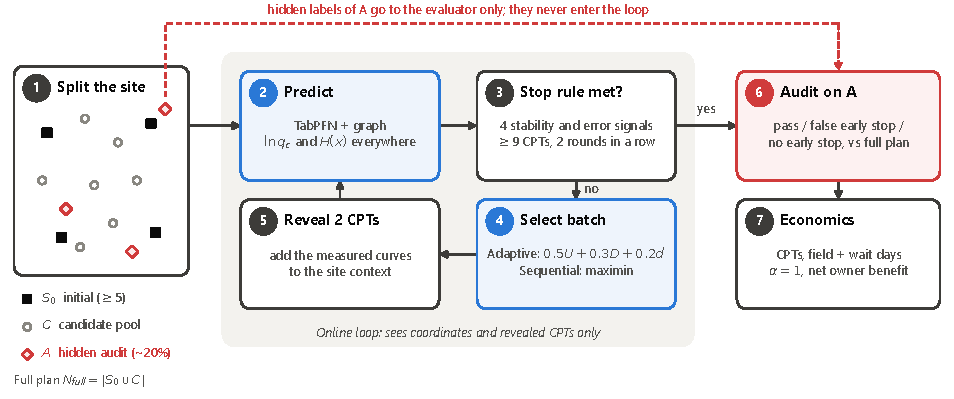
\includegraphics[width=\linewidth]{fig01_workflow.pdf}
\caption{Investigation loop. The hidden audit set $A$ is read only by a separate evaluator after the stop. All
policies share the initial set $S_0$, the candidate pool $C$ and $A$.}
\label{fig:workflow}
\end{figure}

\section{Problem Definition}

At a site with planned CPT positions $x$ and 24 depth cells $z_k = 2.125, 2.375, \dots, 7.875$\,m (each
0.25\,m thick), the regression target is $y(x,z_k)=\ln(\qc/1\,\text{MPa})$. A cell is a \emph{low cell} when
$\qc<1$\,MPa, i.e.\ $y<0$, and the cumulative low-cell thickness at a position is
\begin{equation}
H(x) = 0.25\sum_{k=1}^{24}\mathbb{1}\left[y(x,z_k)<0\right]\quad\text{(m)}.
\end{equation}
Given the revealed CPTs, a model predicts $\hat y(x,z)$ and $\hat H(x)$ at every unrevealed position.
Each site is split into an initial set $S_0$, a candidate pool $C$ and a hidden audit set $A$. Starting from
the revealed set $R=S_0$, a policy repeatedly picks a batch from $C\setminus R$, reveals it, and decides whether
to stop. It seeks the smallest stopping count \Nstop{} for which quality on $A$ meets frozen targets,
compared with completing the full plan of $\Nfull=|S_0\cup C|$ CPTs:
\begin{equation}
\min\ \Nstop\quad\text{s.t.}\quad \text{log-MAE}_A\le\tau_{\log},\ \ \text{thickness-MAE}_A\le\tau_H,\ \
\text{loss relative to the full plan}\le\varepsilon .
\end{equation}

The task therefore combines several problem types: (i)~\emph{spatial regression}: predicting the profile; (ii)~\emph{rare-event classification}: detecting low cells, evaluated with precision, recall, F1 and false-positive rate (FPR, the share of truly non-low cells predicted low); (iii)~\emph{active learning}: choosing informative locations; (iv)~\emph{optimal stopping}: deciding when to stop.

Constraints:
\begin{itemize}
\item \textbf{Information:} only coordinates, planned depths and already revealed curves may enter
  prediction, selection or stopping. Hidden labels are read by a separate evaluator after the stop.
\item \textbf{Grouping:} near-duplicate or repeated soundings form indivisible groups. A nominal batch of
  two can therefore be larger, and all counts are actual positions.
\item \textbf{Small data:} sites, not depth cells or random seeds, are the replicate unit. With four
  evaluation sites the results are descriptive, and no significance tests are claimed.
\item \textbf{No hindsight:} all thresholds are fixed on development sites before evaluation. An online stop
  that fails the audit remains a failure.
\end{itemize}

\section{Dataset Description}

\textbf{Source.} The data come from the public CPT databases of ISSMGE Technical Committee~304
\parencite{tc304}. The Global-CPT collection holds 1,196 soundings from 59 sites or regions
\parencite{ching2023global}. The NL-CPTU/98/2km\textsuperscript{2} set contains the 98 soundings of the New
Lock Terneuzen ship lock in the Netherlands, fully operational since 1~August 2025 \parencite{rws2025terneuzen}.
Only the subset that supports spatial prediction is used (\cref{tab:data}). Of 31 sites, 23 are
\emph{source} sites that only train the models. The 8 \emph{replay} sites, those with at least 20 usable
positions, are split into 4 development and 4 evaluation sites for the decision loop.

\begin{table}[!htb]
\centering\small
\caption{Data hierarchy after screening. Depth cells are repeated measurements within a CPT, not
independent samples.}
\label{tab:data}
\begin{tabularx}{\linewidth}{@{}lrX@{}}
\toprule
Unit & Count & Meaning\\
\midrule
Raw profiles & 503 & CPT curves with coordinates that cover 2--8\,m\\
Distinct planned positions & 495 & repeated soundings at one coordinate merged (8 removed)\\
Usable positions & 492 & complete 24-cell window (3 incomplete profiles removed)\\
Near-duplicate groups & 456 & 435 singletons; groups of 2--5 always move together\\
Sites & 31 & 23 source-only + 8 replay sites (4 development, 4 evaluation)\\
Depth-cell records & 11,808 & $492\times24$ cells of 0.25\,m\\
\bottomrule
\end{tabularx}
\end{table}

\textbf{Features and preprocessing.} Each record carries the site, local coordinates $(x,y)$ in metres,
near-duplicate group, depth and \qc. Each raw curve is interpolated to the 24 cell mid-points, \qc{} is
log-transformed, non-representative repeats are removed and groups are assigned. For New Lock, 80 of the
98 original files are retained: 15 start below 2\,m and 3 end above 8\,m. The neighbour features used by
the models are rebuilt from revealed CPTs only, at every round. They are distances, local medians, low
quantiles, low-cell fractions and vertical gradients.

\textbf{Exploratory analysis.} The 0.25\,m cells lose some thin layers. Against exact threshold crossings of
the raw curves, the cell representation has a thickness MAE of 0.092\,m (90th percentile, P90, 0.256\,m).
498 of 805 raw low intervals thinner than 0.25\,m contain no cell mid-point. All models nevertheless use
the same grid, so comparisons stay fair.

The sites differ sharply (\cref{fig:data}). Wellington Airport is uniformly stiff with no low cells, while
New Lock has 24\% low cells and strong lateral variability. Low cells make up only about 8\% of
source-site cells. Three properties follow: (i)~\emph{small samples per site}, which favour methods that borrow strength across sites or condition on context; (ii)~\emph{spatial correlation}, which favours kernel or neighbour-based models; (iii)~\emph{rare events}, which favour an explicit low-cell decision rather than a median predictor.
These three properties drove the choice of algorithms in \cref{sec:algorithms}.

\begin{figure}[!htb]
\centering
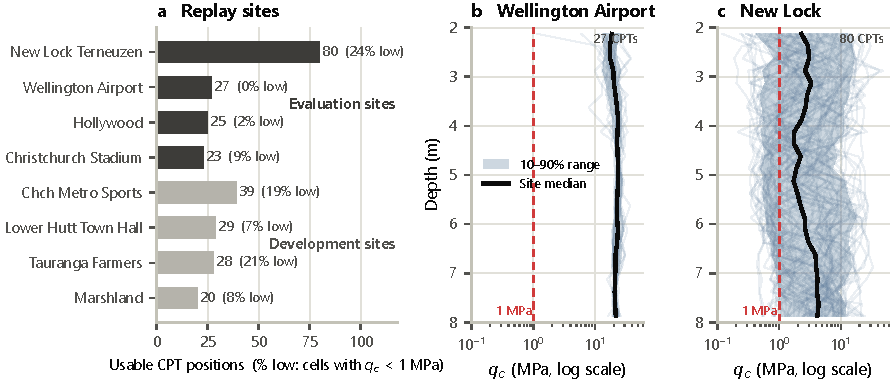
\includegraphics[width=\linewidth]{fig02_dataset.pdf}
\caption{Replay sites and profiles. (a)~Usable CPT positions at the eight replay sites and their share of
low cells ($\qc<1$\,MPa). (b,~c)~All 2--8\,m profiles at the most uniform (Wellington Airport) and most
variable (New Lock) evaluation sites. The band is the 10--90\% range and the black line the site median;
the $x$-axis is logarithmic.}
\label{fig:data}
\end{figure}

\section{Algorithm Selection and Rationale}\label{sec:algorithms}

All five predictors receive the same revealed CPTs at every state. Thickness and low-cell labels are derived
from each method's single predicted curve.

\textbf{Gaussian process (GP).} A GP is a prior over functions defined by a kernel. Its prediction is a
kernel-weighted combination of the observations, and its variance grows away from them
\parencite{rasmussen2006gp}. We use an anisotropic Mat\'ern-3/2 kernel on residuals from a source-site depth
trend, refitted each round. It gives native uncertainty, but its smoothness blurs thin low layers.

\textbf{XGBoost residual.} Gradient boosting adds regression trees one at a time, each fitted to the current
residuals \parencite{chen2016xgboost}. Here the trees correct an inverse-distance (IDW) estimate using 24
neighbour features. This captures non-linear local effects, but the trees are fixed after source training.

\textbf{Conditional neural process (CNP).} A CNP encodes the revealed profiles relative to the query, pools
them in a permutation-invariant way and decodes a full profile \parencite{garnelo2018cnp}. It learns
cross-site transfer, but its L1 loss targets the median, so rare low cells are smoothed away.

\textbf{TabPFN.} A Transformer pre-trained on synthetic tabular tasks predicts by in-context learning: the
site's revealed rows are passed as context, with no gradient step per round \parencite{hollmann2025tabpfn}.
We fine-tuned it on source sites and then froze it. Two hybrids are tested. \emph{TabPFN joint} blends a
TabPFN residual with a triangulation estimate and decides low cells per whole profile. \emph{TabPFN + graph}
blends it with a robust graph interpolation and labels a cell low if either branch does, favouring recall.

\textbf{Compare and contrast.} Each method trades off differently:
\begin{itemize}
\item GP needs no source data and gives uncertainty, but assumes smooth ground.
\item XGBoost and TabPFN exploit cross-site patterns.
\item TabPFN also adapts to a new site without retraining.
\item CNP is the most data-hungry.
\end{itemize}
Kriging is close to the GP. Entropy-based sampling \parencite{guan2022adaptive} targets liquefaction, not
\qc{} profiles. Reinforcement learning was rejected because four evaluation sites cannot support a learned
policy.

\textbf{Division of labour.} The primary predictor was chosen in advance by the lowest development
log-MAE: TabPFN + graph (0.578), ahead of XGBoost (0.597) and TabPFN joint (0.598). It drives prediction and
stopping; the GP supplies uncertainty and XGBoost a second opinion.

\section{Methodology}

\subsection{Evaluation design}
The loop in \cref{fig:workflow} is replayed on historical data in a three-level, site-held-out design.
\begin{enumerate}
\item \emph{Source training.} In each of three folds the models are trained on source sites. Checkpoints
  and early stopping are chosen on that fold's validation sites.
\item \emph{Development.} Four replay sites select the primary model, the acquisition weights and the stop
  thresholds: Lower Hutt Town Hall, Tauranga Farmers, Christchurch Metro Sports and Marshland.
\item \emph{Evaluation.} Four replay sites test the frozen configuration: Wellington Airport, Christchurch
  Stadium, Hollywood and New Lock. Each is predicted with the fold weights that excluded it from both
  training and checkpoint selection.
\end{enumerate}

For every site and seed (17, 29, 43), whole groups are assigned to the audit set $A$ ($\approx$20\%), a
spatially dispersed $S_0$ ($\geq$5 positions) and the candidate pool $C$. Three policies share each split:
\begin{itemize}
\item \textbf{Full plan} (\Bfull) completes every position in $S_0\cup C$; this is the engineering reference.
\item \textbf{Sequential} (\Bseq) adds the two candidates that maximise the minimum distance to any
  revealed CPT. This \emph{maximin} rule is a space-filling baseline. It applies the stop rule.
\item \textbf{Adaptive} (\Padapt) adds the two candidates with the highest acquisition score and applies the
  same stop rule.
\end{itemize}
Full versus Adaptive measures the total benefit. Sequential versus Adaptive isolates what intelligent
location choice adds beyond simply stopping early. The evaluation therefore comprises 4~sites $\times$
3~seeds $\times$ 2~stopping policies $=24$ trajectories, plus 12 full-plan runs.

\textbf{Metrics.} All metrics are computed on $A$. (i)~\emph{log-MAE} is the mean $|\hat y-y|$ over audit cells; (ii)~\emph{thickness MAE} is the mean $|\hat H-H|$ over audit positions; and (iii)~the \emph{low-cell
metrics} are precision, recall, F1 and FPR.
Values are averaged within seed, then within site, and then equally across sites (the \emph{equal-site
mean}).

\subsection{Acquisition score}
For each candidate group the policy computes three signals: (i)~$U$, the mean GP predictive standard deviation of $\ln\qc$; (ii)~$D$, the share of cells where the primary model and XGBoost disagree on $\qc<1$\,MPa; (iii)~$d$, the distance to the nearest revealed CPT.
Each signal is converted to a 0--1 rank within the pool, and the score is
\begin{equation}
a(x)=0.5\,\mathrm{rank}(U)+0.3\,\mathrm{rank}(D)+0.2\,\mathrm{rank}(d).
\end{equation}
The weights are an engineering heuristic: uncertainty first, model disagreement second and spacing as a
tie-breaker. The only alternative tried omitted disagreement (0.7,~0,~0.3). Within a batch only $d$ is
updated after each pick, so the second choice is pushed away from the first without seeing its curve.

\subsection{Online stopping and independent audit}
Each round, the controller computes four signals on a fixed grid of all planned positions $\times$ 24
depths:
\begin{itemize}
\item the 90th percentile over grid cells of the round-to-round change in predicted $\ln\qc$ ($\Delta Q_{90}$);
\item the 90th percentile over positions of the change in predicted thickness ($\Delta H_{90}$);
\item a leave-group-out log-MAE on up to five initial groups;
\item the 90th percentile of the GP standard deviation.
\end{itemize}
The controller stops when all four pass for two consecutive rounds, provided at least nine CPTs are revealed
and every populated quadrant of the site is covered. Because batches add two CPTs, the earliest possible
stop is at 11~CPTs. Thresholds were set as quantiles (0.50/0.75/0.90) of the signals at acceptable
development states. The 0.50 quantile was selected because it maximised verified saving minus false-stop
rate; the 0.75 and 0.90 quantiles gave development false-stop rates of 17\% and 58\%.

The audit has two parts: (i)~\emph{absolute targets} of log-MAE $\le0.626$ and thickness MAE $\le0.881$\,m,
the development full-plan 75th percentiles plus fixed margins; and (ii)~a \emph{relative tolerance} of no
more than 0.05 log-MAE or 0.25\,m worse than the full plan.
Low-cell recall $\ge0.5$ with FPR $\le0.1$ is audited separately as a diagnostic.

\subsection{Hyperparameters}
\Cref{tab:hyper} lists every setting. Model settings were fixed during source training on validation sites.
Decision settings were fixed on development sites. No setting was tuned on evaluation sites.

\begin{table}[!htb]
\centering\small
\caption{Hyperparameters and how they were chosen.}
\label{tab:hyper}
\begin{tabularx}{\linewidth}{@{}lX@{}}
\toprule
Component & Setting (selection)\\
\midrule
GP & Mat\'ern $\nu=3/2$, anisotropic length scales initialised at (20, 20, 1)\,m, white-noise term; refitted
  by marginal likelihood each round\\
XGBoost residual & 3-NN IDW base (power 2) + $w\times$trees; 24 features; depth 6, learning rate 0.3,
  early stopping (36--37 trees); $w\in\{0, 0.25, 0.5, 1\}$ chosen per fold (0.25, 0.25, 0.5)\\
CNP & 64 hidden units, mean + max pooling, L1 loss on $\ln\qc$; 26,817 parameters; 500--1,200 steps,
  checkpoint by validation log-MAE\\
TabPFN & v2 weights (package 9.2.0), 1 estimator; fine-tuned with CRPS (continuous ranked probability score)
  + MSE, 500--600 updates; joint blend 0.5/0.5\\
Graph branch & 4 nearest neighbours, vertical weight 0.15, pseudo-Huber $\delta=0.35$\\
Acquisition & weights (0.5, 0.3, 0.2); batch of 2 groups; alternative (0.7, 0, 0.3) rejected on development\\
Stop rule & $\geq$9 CPTs, 2 rounds; $\Delta Q_{90}\le0.082$, $\Delta H_{90}\le0$\,m, support log-MAE
  $\le0.584$, GP-std P90 $\le0.461$ (0.50 quantile of development signals)\\
Experiment & seeds 17, 29, 43; audit share $\approx$20\%; $|S_0|\ge5$\\
\bottomrule
\end{tabularx}
\end{table}

\subsection{Economic model}
The owner's net benefit of a policy relative to the full plan is
\begin{equation}
B_{\text{net}}=(C_{\text{full}}-C_{\text{policy}})+\alpha\,\Delta T_{\text{inv}}\,(c_{\text{day}}+b_{\text{day}})-C_{\text{AI}},
\end{equation}
where the terms are: (i)~$C$ is investigation cost (\eur{750} per CPT, all-in); (ii)~$\Delta T_{\text{inv}}$ is the calendar days saved: 5 CPTs per rig-day with one rig, converted at 7/5, plus a 0.25-day decision delay at every batch transition; (iii)~$c_{\text{day}}=\eur{5,000}$ is the avoidable project cost per day; (iv)~$b_{\text{day}}=\eur{3,000}$ is the owner's benefit per day of earlier opening; (v)~$C_{\text{AI}}=\eur{600}$ is deployment and review per run.
In the main scenario $\alpha=1$, meaning every investigation day saved shortens the project. $\alpha=0.5$ and
0.75 are sensitivity cases, alongside one-at-a-time parameter ranges. A failed early stop would be repaired
to the full plan, with remobilisation (\eur{560}) and two days' delay.

Only the remobilisation cost and the consultant rate behind $C_{\text{AI}}$ come from a 2025 Dutch quotation
\parencite{mos2025quote}. All other values are explicit assumptions, following cost- and
schedule-estimating guidance \parencite{gao2015schedule,gao2020cost}. The same Dutch-based values are
applied to every site; for non-Dutch sites this is a standardised transfer, not local evidence.

\subsection{Tools and libraries}
The implementation uses Python 3.11, NumPy 2.4, pandas 3.0 and SciPy 1.17, scikit-learn 1.9 for the GP \parencite{pedregosa2011sklearn}, XGBoost 3.2, PyTorch 2.11 for the CNP, TabPFN 9.2.0 \parencite{priorlabs_tabpfn} and matplotlib.
Models ran on an NVIDIA RTX 4080 (16\,GB).

\section{Implementation}

The code is a Python package (\texttt{cpt\_budget}) whose modules mirror the information boundary:
\begin{itemize}
\item data splits;
\item models with a common \texttt{condition(revealed)}/\texttt{predict(query)} interface, which strips
  queries of measured values;
\item acquisition and stop rule;
\item replay loop;
\item a separate audit evaluator;
\item economics.
\end{itemize}
The frozen configuration stores SHA-256 fingerprints of data, weights and settings. The core of batch
selection is:
\begin{lstlisting}
while remaining and chosen_count < batch_size:
    dist  = [min_distance(g, observed_xy) for g in remaining]
    score = 0.5*group.rank_U + 0.3*group.rank_D + 0.2*rank01(dist)
    gid   = argmax(score)                         # ties: group id, then location id
    chosen += members(gid)                        # whole near-duplicate group
    observed_xy = vstack([observed_xy, xy(gid)])  # coordinates only, never curves
\end{lstlisting}
Each round is logged; for example, the adaptive run at Wellington Airport (seed 17) stops in round 3:
\begin{lstlisting}[style=output]
round n_obs dQ90  dH90 support_logMAE gp_std_P90 streak stop
  3    11   0.067 0.00     0.132        0.169      2    online_stability
\end{lstlisting}
\textbf{Key decisions.} TabPFN weights stay frozen, so each round only updates the context and takes
seconds. Grouping is enforced throughout. All 14 CNP and 129 TabPFN weight tensors differ from
initialisation, so weak CNP results are not an untrained-model artefact.

\textbf{Checks.} Automated checks show that audit labels cannot affect predictions (24 paired contexts,
difference 0). They also confirm that group counts are exact, inputs are unchanged and economic sums
recompute. All 95 unit tests pass.

\section{Results and Evaluation}

\subsection{Prediction quality of the five methods}

\begin{table}[!htb]
\centering\small
\caption{Prediction quality (equal-site means over registered observation states). $^{\dagger}$Primary model,
selected on development log-MAE. Bold marks the best of the five main methods per column; CNP's 0\% FPR is
not bolded because it never predicts a low cell. Recall excludes Wellington Airport, which has no low cells.}
\label{tab:prediction}
% generated by report/make_tables.py -- do not edit by hand
\begin{tabular}{@{}lrrrrrrr@{}}
\toprule
 & \multicolumn{2}{c}{Development (4 sites)} & \multicolumn{5}{c}{Evaluation (4 sites)}\\
\cmidrule(lr){2-3}\cmidrule(l){4-8}
Method & log-MAE & Thick.\ (m) & log-MAE & Thick.\ (m) & Recall (\%) & FPR (\%) & F1\\
\midrule
GP & 0.658 & 0.614 & 0.509 & \textbf{0.400} & 14.0 & \textbf{1.9} & 0.11\\
XGBoost residual & 0.597 & 0.571 & 0.512 & 0.485 & 31.2 & 6.9 & 0.30\\
CNP & 0.833 & 0.774 & 0.657 & 0.430 & 0.0 & 0.0 & 0.00\\
TabPFN joint & 0.598 & \textbf{0.483} & \textbf{0.497} & 0.491 & 33.3 & 7.8 & 0.30\\
TabPFN + graph$^{\dagger}$ & \textbf{0.578} & 0.586 & 0.503 & 0.595 & \textbf{36.3} & 9.6 & \textbf{0.31}\\
\midrule
\multicolumn{8}{l}{\textit{TabPFN ablation (the fine-tuned joint row above completes the set)}}\\
\quad Residual, pretrained weights & 0.627 & 0.642 & 0.506 & 0.494 & 23.4 & 5.9 & 0.23\\
\quad Residual, fine-tuned weights & 0.598 & 0.626 & 0.502 & 0.509 & 22.4 & 6.0 & 0.22\\
\quad Residual, fine-tuned + sign guard & 0.598 & 0.573 & 0.503 & 0.497 & 32.1 & 7.3 & 0.30\\
\quad Joint, pretrained weights & 0.604 & 0.485 & 0.495 & 0.480 & 34.9 & 7.5 & 0.32\\
\bottomrule
\end{tabular}

\end{table}

\textbf{Main comparison.} TabPFN joint has the lowest evaluation profile error (\cref{tab:prediction}): 0.497,
2.9\% below XGBoost. TabPFN + graph is 1.8\% below XGBoost. The margins are small and site-dependent. Joint
beats XGBoost in 9 of 12 site--seed cells, by 0.9--3.9\% per site. At New Lock the GP is better than every
TabPFN hybrid (0.976 against 1.034). On evaluation sites the GP has the lowest thickness error (0.400\,m),
but mainly because it rarely predicts low cells: its recall is 14\%. On development sites its thickness
error is the second worst. The graph union buys the highest recall (36\%), at the cost of the highest FPR
(9.6\%) and the largest thickness error. CNP never predicts $\qc<1$\,MPa, a genuine negative result for a
median-trained set model on rare events.

\textbf{Site difficulty.} Site difficulty dominates model differences (\cref{fig:models}): log-MAE is
0.11--0.24 at Wellington Airport and 0.98--1.14 at New Lock.

\textbf{TabPFN ablation.} Source-site fine-tuning lowered the raw residual's development log-MAE from 0.627
to 0.598. On evaluation sites, however, the pretrained and fine-tuned joint models differ by under 0.002.
Most of the thickness gain comes from the spatial blend and the whole-profile decision (development 0.626
$\rightarrow$ 0.483\,m), not from the Transformer weights. The improvement belongs to the hybrid, not to
TabPFN alone.

\textbf{Error analysis.} In the full-plan predictions at New Lock, error peaks at 4--6\,m, where 23\% of cells are low.
In that band the primary model recovers 53\% of low cells but raises 85 false alarms. The GP flags only 1--3\%
of cells as low, against 9--23\% true, so it under-predicts soft layers throughout. Thin layers below the
0.25\,m grid add irreducible error.

\begin{figure}[!htb]
\centering
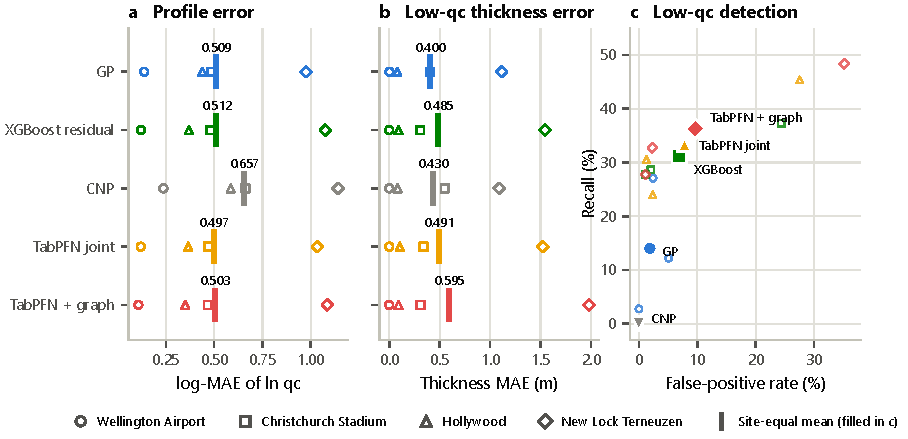
\includegraphics[width=\linewidth]{fig04_five_models.pdf}
\caption{Five AI methods on identical observation states at the four evaluation sites. Open marks are site
means (shape = site), and bars and filled circles are equal-site means. (c)~Low-cell recall against FPR;
recall is undefined at Wellington Airport.}
\label{fig:models}
\end{figure}

\subsection{Selection, stopping and audit}

\begin{figure}[!htb]
\centering
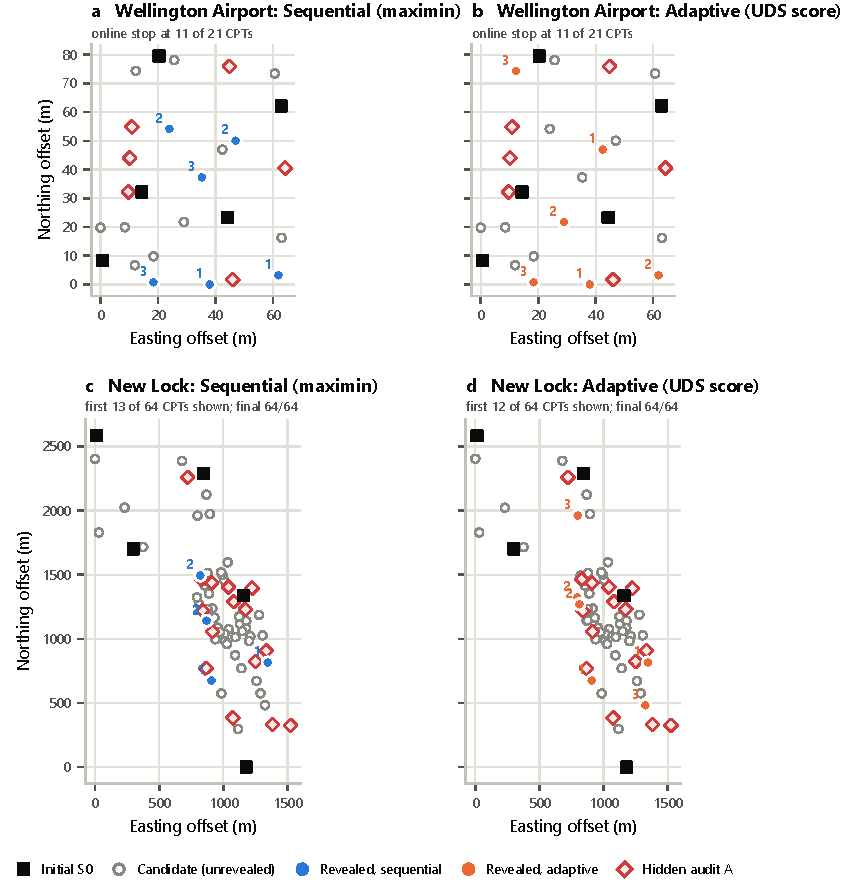
\includegraphics[width=0.62\linewidth]{fig03_selection_maps.pdf}
\caption{Selection maps, seed 17. (a,~b)~Wellington Airport at the online stop. (c,~d)~New Lock after the
first 12--13 CPTs. Numbers give the round in which a position was revealed. The adaptive score combines GP
uncertainty $U$, model disagreement $D$ and distance $d$.}
\label{fig:maps}
\end{figure}

\textbf{Where each policy samples.} The adaptive score does choose different locations from maximin
(\cref{fig:maps}). At New Lock it concentrates on the dense, variable central cluster where uncertainty and
disagreement are high, whereas maximin spreads out.

\textbf{Quality as CPTs are added (\cref{fig:quality}).} At the three easier sites audit quality is inside
the targets from the first few CPTs. At New Lock the error falls steeply over the first 15 CPTs and then
plateaus at log-MAE $\approx0.9$ and thickness MAE $\approx1.1$--1.5\,m, above both targets, even with all
64 CPTs.

\begin{table}[!htb]
\centering\small
\caption{Decision outcomes at the evaluation sites (means of three seeds). $|A|$ is the number of audit
positions. ``Full plan passes'' counts the seeds in which even the full plan meets the audit targets.
Oracle~$N$ is the smallest adaptive count that would have passed, found with hindsight; it is a
diagnostic, not a policy. Net is the owner's benefit of the adaptive policy at $\alpha=1$.}
\label{tab:decisions}
% generated by report/make_tables.py -- do not edit by hand
\begin{tabular}{@{}lrrrrrrrrr@{}}
\toprule
 & & & \multicolumn{2}{c}{CPTs at stop} & \multicolumn{2}{c}{Saving (\%)} & Full plan & Oracle & Net\\
\cmidrule(lr){4-5}\cmidrule(lr){6-7}
Site & $N_{\text{full}}$ & $|A|$ & Seq. & Adapt. & Seq. & Adapt. & passes & $N$ (adapt.) & k\euro\\
\midrule
Wellington Airport & 21 & 6 & 11.0 & 11.0 & 47.6 & 47.6 & 3/3 & 9 & +23.3\\
Christchurch Stadium & 18 & 5 & 18.0 & 18.0 & 0.0 & 0.0 & 3/3 & 9 & $-$12.6\\
Hollywood & 20 & 5 & 18.7 & 20.0 & 6.7 & 0.0 & 3/3 & 13--14 & $-$11.9\\
New Lock & 64 & 16 & 64.0 & 64.0 & 0.0 & 0.0 & 0/3 & none & $-$55.9\\
\midrule
Equal-site mean &  &  &  &  & 13.6 & 11.9 &  &  & $-$14.3\\
\bottomrule
\end{tabular}

\end{table}

\textbf{Stopping outcomes.} No early stop failed the audit (\cref{tab:decisions}, \cref{fig:outcomes}), but
the evidence is thin. Only 7 of the 24 evaluation trajectories stopped early: 6 at Wellington Airport,
where every audited state passes, and 1 at Hollywood (Sequential, seed~17). The rule's real value is that
it never stopped at New Lock, where every early stop would have failed. A naive rule that stops at the
ninth CPT would have made 7 false stops (all six New Lock runs plus one at Hollywood). Ablations show that
the leave-group-out support error carries this safety: without it the evaluation runs make 3 (Sequential)
and 2 (Adaptive) false stops, whereas dropping any other signal adds none.

\textbf{Savings.} Equal-site savings were 13.6\% (Sequential) and 11.9\% (Adaptive). Wellington Airport,
21\,$\rightarrow$\,11 CPTs (47.6\%), is the only adaptive saving, and Sequential saved exactly the same
there. Eleven CPTs is the earliest stop the rule allows, so this saving reflects how uniform the site is,
not fine-grained learning.

\textbf{Adaptive against Sequential.} Adaptive location choice showed no detectable advantage. Across all
24 site--seed pairs on the eight replay sites, the two policies' stopping counts differed only 3 times, and
in both directions. At matched CPT counts the sign of the audit-error difference varies across sites and
seeds.

\textbf{Low cells and audit size.} The low-cell targets (recall $\ge0.5$, FPR $\le0.1$) failed at all three
sites that contain low cells. Audit sets are small (5--6 positions, 16 at New Lock), which limits every
site-level verdict.

\begin{figure}[!htb]
\centering
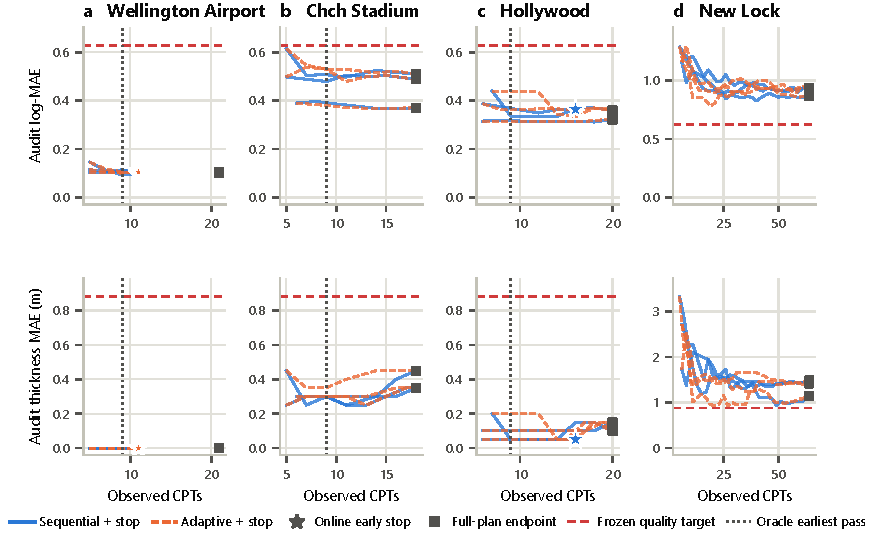
\includegraphics[width=\linewidth]{fig05_quality_vs_cpts.pdf}
\caption{Hidden-audit quality as CPTs are added (three seeds per policy). Stars mark online early stops,
squares the full plan, red dashed lines the frozen targets, and dotted lines the earliest passing count
found with hindsight (none at New Lock). Step changes reflect the small audit sets.}
\label{fig:quality}
\end{figure}

\begin{figure}[!htb]
\centering
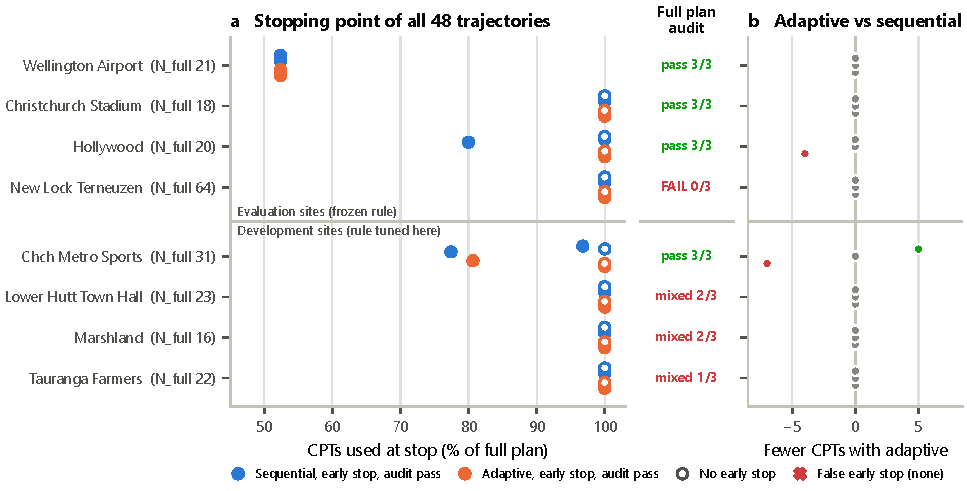
\includegraphics[width=\linewidth]{fig06_site_outcomes.pdf}
\caption{Stopping points of all 48 Sequential and Adaptive trajectories (8 sites $\times$ 3 seeds $\times$ 2
policies). (a)~CPTs used at the stop, with the full-plan audit verdict per site. (b)~CPTs saved by Adaptive
relative to Sequential, paired by seed.}
\label{fig:outcomes}
\end{figure}

\textbf{The rule is safe but conservative.} With hindsight, Christchurch Stadium already met the targets
with 9 of 18 CPTs, and Hollywood with 13--14 of 20 (Adaptive). Yet both Adaptive runs went to the full plan.
No single signal is to blame. At Christchurch Stadium, $\Delta Q_{90}$ and the GP uncertainty block the
most rounds; at Hollywood, $\Delta Q_{90}$ and $\Delta H_{90}$ block about equally often. $\Delta H_{90}\le0$ allows changes at up to 10\% of positions. Its
value of zero is a quantile tie in the development data, not a deliberately chosen tolerance. GP
uncertainty was only weakly related to actual audit error on evaluation sites (mean Spearman $\rho=0.21$,
against 0.60 on development sites).

\subsection{Economic value}

\textbf{Wellington Airport.} The observed counts were priced in the scenario (\cref{fig:econ}). The adaptive
policy yields $+$\eur{23,300}: (i)~\eur{7,500} from ten avoided CPTs; (ii)~\eur{10,250} of avoided project cost and \eur{6,150} of earlier-opening benefit, from finishing 2.05 days earlier; (iii)~less \eur{600} of AI cost.
Sequential stopping earns the same amount, so this benefit comes from staged stopping, not from AI location
choice.

\textbf{Other sites.} The other three sites are negative, from $-$\eur{11,900} to $-$\eur{55,900}, although
they used no extra CPTs. The staged campaign adds a 0.25-day decision delay at every batch transition. At
New Lock there are 27--29 transitions, which delay completion by 6.9 days. With zero delay these losses
shrink to the \eur{600} AI cost. With a one-day delay New Lock would lose \eur{222,000}, and Wellington
Airport would still gain \eur{5,300}. Across all four evaluation sites the mean is $-$\eur{14,300} for
Adaptive and $-$\eur{13,500} for Sequential.

\textbf{Sensitivity.} At $\alpha=0.5$ Wellington Airport falls to \eur{15,100}. No site changes sign within
any tested range.

\begin{figure}[!htb]
\centering
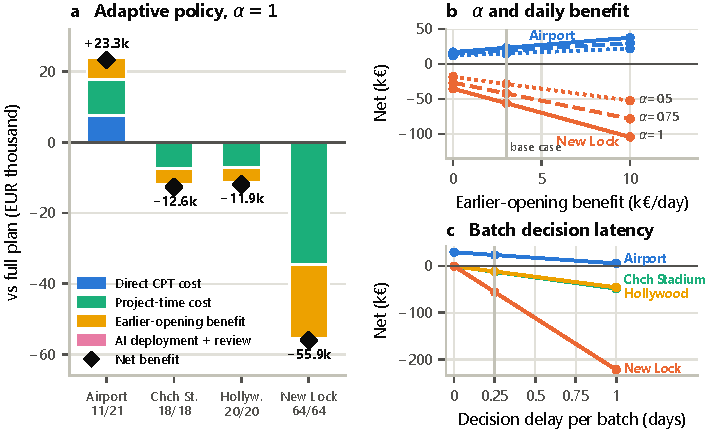
\includegraphics[width=\linewidth]{fig07_economics.pdf}
\caption{Owner's financial scenario, EUR 2025, Adaptive policy (mean of three seeds). (a)~Benefit components
relative to the full plan at $\alpha=1$. (b)~Net benefit as $\alpha$ and the daily earlier-opening benefit
vary (Wellington Airport and New Lock; the vertical line marks the base case). (c)~Net benefit against the
decision delay per batch.}
\label{fig:econ}
\end{figure}

\section{Discussion and Insights}

\textbf{What worked.} The pipeline is auditable. Hidden labels never reach the controller, every stop is
audited, and all trajectories are reported, including failures. No leakage was found by the automated
checks. The stop rule vetoed every stop at the one site where stopping would have failed. The TabPFN
hybrids were competitive, giving the best profile error and low-cell recall. The GP remained the most
conservative low-cell detector and the source of the uncertainty signal.

\textbf{What the results reveal.} Four lessons emerge.
\begin{enumerate}
\item \emph{Site predictability, more than the algorithm, decided whether CPTs could be saved.} Savings
  appeared only where five CPTs already describe the ground, and vanished at New Lock, where even 64 CPTs
  leave log-MAE near 0.9.
\item \emph{Location choice added nothing measurable here.} The benefit came from staged investigation
  combined with a stopping rule.
\item \emph{Model choice matters less than the decision it serves.} The five predictors lie within about
  3\% of each other on profile error. Their low-cell behaviour, however, differs sharply: GP is
  conservative, the graph hybrid sensitive and CNP blind. This difference changes what a stop rule can
  safely conclude.
\item \emph{Time, not CPT price, dominates the economics.} Per-batch decision delay can turn a neutral
  outcome strongly negative. A deployed system must return decisions within the working day, and should
  recommend the full plan early when a site is clearly unpredictable.
\end{enumerate}

\textbf{Threats to validity.}
\begin{itemize}
\item \emph{Optimistic development data.} The four development sites served as checkpoint-selection
  (validation) sites during source training. This likely explains why the learned models beat the GP by
  12\% on development sites but by only 1\% on evaluation sites. It also means the model ranking (0.578 vs
  0.597) is within noise.
\item \emph{Prior exposure.} The evaluation sites had been inspected in an earlier project stage, so this
  is a site-held-out re-evaluation, not a blind test.
\item \emph{Small samples.} With four evaluation sites, 5--16 audit positions per site and seeds that share
  the same ground, all conclusions are descriptive. The 7 observed early stops give a 95\% upper bound of
  roughly 40\% on the false-stop rate.
\item \emph{Confounding at New Lock.} New Lock is the only non-New-Zealand site, the largest site, and has
  no close source analogue. Domain shift, size and heterogeneity cannot be separated there.
\item \emph{Economic assumptions.} The economics rest on assumed unit values and on $\alpha=1$, which places
  investigation on the critical path.
\item \emph{Representation and labels.} The 0.25\,m grid misses thin layers, and the 1\,MPa threshold is a
  research indicator.
\end{itemize}

\textbf{Future improvements.} (i)~learn quality-predictive stop signals, rather than fixed quantile thresholds, so that the clear opportunities at Christchurch Stadium and Hollywood are taken; (ii)~add a site-predictability check after the initial CPTs that recommends the full plan at once for New Lock-like sites; (iii)~use larger batches or same-day decisions to cut latency; (iv)~use an event-weighted loss and a 0.1\,m grid for low-cell detection; (v)~evaluate on genuinely new sites with real contract and programme data.
A post-evaluation exploration (not used for any claim above) tried variance-reduction acquisition at New
Lock. It lowered the GP's budget-averaged profile error by about 11\% relative to maximin but worsened
thickness error, and none of 432 explored states met the targets.

\section{Conclusion}

\textbf{What was built.} We built and audited an end-to-end, AI-guided CPT investigation loop. It combines
five AI predictors, an uncertainty--disagreement--distance acquisition score, a multi-signal stop rule and
an owner's economic model.

\textbf{Findings.} (i)~the TabPFN hybrids gave the lowest profile error (0.497 log-MAE) and the highest low-cell recall (36\%), within about 3\% of XGBoost and GP; (ii)~with rules frozen on development sites, no early stop failed the audit; (iii)~CPTs were saved only at the most uniform site: 47.6\%, at the minimum the rule allows, worth $+$\eur{23,300} in the main scenario; (iv)~adaptive location choice did not beat simple maximin ordering; (v)~New Lock could not reach the quality targets with any number of CPTs.

\textbf{Lessons.} An AI algorithm should be judged by the decision it supports, using an independent audit
and reporting negative results. In investigation planning, site predictability and decision latency
mattered more here than the marginal accuracy of the predictor.


\section{References}
\printbibliography[heading=none]

\end{document}
